\documentclass[pdftex,12pt,xcolor=svgnames]{beamer}

\mode<presentation>
{
  \usetheme{boxes}
  \usecolortheme[named=MidnightBlue]{structure}
  %\setbeamercolor{normal text}{bg=NavajoWhite!20}
  %% \usefonttheme{serif}
  \setbeamertemplate{navigation symbols}{}
  % Show frame number and author name in footline
  \setbeamertemplate{frametitle}[default][center]
  \setbeamertemplate{footline}[frame number]
  \setbeamertemplate{items}[circle]
  %\addtobeamertemplate{footline}{\quad\textcolor{gray}{James Robert Lloyd}}{}
  % Set frame titles in small capitals
  %% \setbeamerfont{frametitle}{shape=\scshape,family=\rmfamily,size={\fontsize{16}{20}}}
  %% \setbeamercolor{frametitle}{bg=gray!60!white,fg=black}
  %% \setbeamercolor{frametitle}{bg=blue,fg=black}
  % Alerted text: blue (uncomment second line if theme sets alerted text to bold)
  \setbeamercolor{alerted text}{fg=blue}
  %\setbeamerfont*{alerted text}{}
  \setbeamertemplate{bibliography item}[text] %{\hbox{\donotcoloroutermaths$\blacktriangleright$}}
  \setbeamertemplate{bibliography entry title}{}
  \setbeamertemplate{bibliography entry author}{}
  \setbeamertemplate{bibliography entry note}{}
  \setbeamertemplate{bibliography entry location}{}

}
\usepackage[english]{babel}
\usepackage[latin1]{inputenc}
\usepackage{times}
\usepackage[T1]{fontenc}
\usepackage{hyperref}
\usepackage{multimedia}
\usepackage{eepic}
\usepackage{graphicx}
%\usepackage[nohug]{latexinclude/diagrams}
\usepackage{tikz}
\usetikzlibrary{calc}

%% \newcommand{\footlineextra}[1]{
%%     \begin{tikzpicture}[remember picture,overlay]
%%         \node[yshift=1.5ex,anchor=south east] at (current page.south east)
%% {#1};
%%     \end{tikzpicture}
%% }

\newcommand{\footlineextra}[1]{
    \begin{tikzpicture}[remember picture,overlay]
        \node[xshift=-5ex,yshift=-0.5ex,anchor=south east] at (current page.south east)
             {\mbox{\tiny \textcolor{MidnightBlue}{#1}}};
    \end{tikzpicture}
}

\def\sectionframe#1{
  {
    \setbeamertemplate{footline}{\empty}
    \begin{frame}{}
      \begin{center}
        \huge\sc #1
      \end{center}
    \end{frame}
  }
}


\usepackage{etex}
\usepackage{tabularx}
\usepackage{include/picins}
\usepackage{include/preamble}
\usepackage{setspace}
\usepackage{xcolor}
\usepackage{tikz}
\usepackage{listings}
%\usepackage{algorithm}
%\usepackage{algpseudocode}

\definecolor{Blue}{rgb}{0.0,0.0,1.0}
\lstloadlanguages{Python}%
\lstset{language=Python,
        frame=none,
        basicstyle=\tiny\ttfamily\bfseries,
        keywordstyle=[1]\color{Blue},
        keywordstyle=[2]\color{Purple},
        commentstyle=\usefont{T1}{pcr}{m}{sl}\color{Green},
        keepspaces=true,
        }
\lstset{language=Python} 

\setlength{\columnsep}{0.03\textwidth}
\setlength{\columnseprule}{0.0018\textwidth}
\setlength{\parindent}{0.0cm}
\hypersetup{colorlinks=true,citecolor=blue}
\newcommand{\paren}[1]{\left( #1 \right)}
\newcommand{\vv}{\mathbf{v}}

\title{Early Stopping as Nonparametric Variational Inference}

\author{
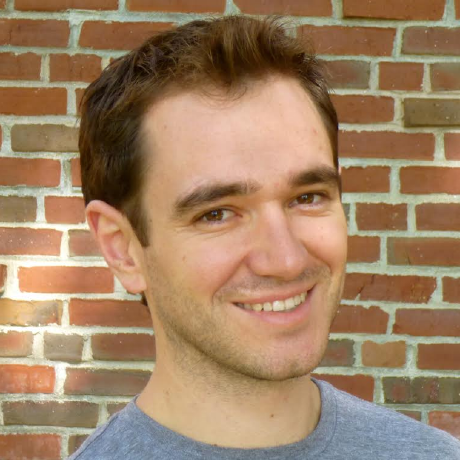
\includegraphics[height=0.16\textwidth]{talkfigs/dougal}
\qquad\qquad
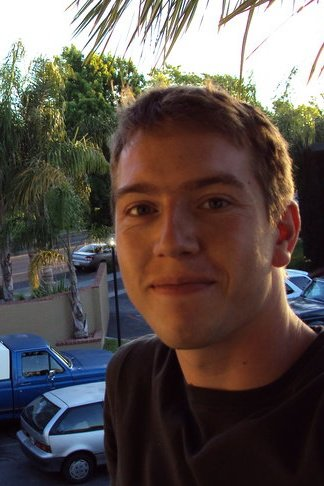
\includegraphics[height=0.16\textwidth, trim=20mm 25mm 0mm 25mm, clip]{talkfigs/david2}
\qquad\qquad
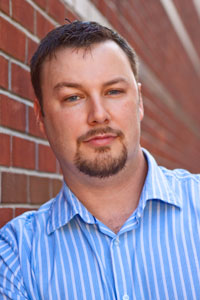
\includegraphics[height=0.16\textwidth]{talkfigs/adams}
\\
Dougal Maclaurin, David Duvenaud, Ryan Adams}

\institute{Harvard University}

\begin{document}

\frame[plain] {\titlepage}

\newcommand{\trail}[3]{\includegraphics<#3>[width=6cm]{../experiments/2015_03_02_funnel/5-talk/figures/trails_#1/iter_#2.pdf}}%
\newcommand{\trixa}{0}%
\newcommand{\trixb}{12}%
\newcommand{\trixc}{6}%

\frame[plain]{\frametitle{Optimization as Inference}
\begin{columns}
\hspace{-1cm}\begin{column}{6cm}
\begin{itemize} 
  \item Optimization paths start from random init, and converges to modes...
\end{itemize}
\end{column}
\begin{column}{5cm}
\trail{\trixa}{0}{1}%
\trail{\trixa}{1}{2}%
\trail{\trixa}{2}{3}%
\trail{\trixa}{3}{4}%
\trail{\trixa}{4}{5}%
\trail{\trixa}{5}{6}%
\trail{\trixa}{6}{7}%
\trail{\trixa}{7}{8}%
\trail{\trixa}{8}{9}%
\trail{\trixa}{9}{10}%
\trail{\trixa}{10}{11}%
\trail{\trixb}{0}{12}%
\trail{\trixb}{1}{13}%
\trail{\trixb}{2}{14}%
\trail{\trixb}{3}{15}%
\trail{\trixb}{4}{16}%
\trail{\trixb}{5}{17}%
\trail{\trixb}{6}{18}%
\trail{\trixb}{7}{19}%
\trail{\trixb}{8}{20}%
\trail{\trixb}{9}{21}%
\trail{\trixb}{10}{22}%
\trail{\trixc}{0}{23}%
\trail{\trixc}{1}{24}%
\trail{\trixc}{2}{25}%
\trail{\trixc}{3}{26}%
\trail{\trixc}{4}{27}%
\trail{\trixc}{5}{28}%
\trail{\trixc}{6}{29}%
\trail{\trixc}{7}{30}%
\trail{\trixc}{8}{31}%
\trail{\trixc}{9}{32}%
\trail{\trixc}{10}{33}%
\end{column}
\end{columns}}

\newcommand{\dist}[2]{\includegraphics<#2>[width=6cm]{../experiments/2015_03_02_funnel/6-nicer/figures/dists_#1.pdf}}%

\frame[plain]{\frametitle{Main Idea}
\begin{columns}
\hspace{-1cm}\begin{column}{6cm}
\begin{itemize} 
\item What about the implicit distribution of parameters after optimizing for $t$ steps?
\item Starts as a bad approximation (prior dist)
\item Ends as a bad approximation (point mass)
\item Choosing best intermediate dist $=$ early stopping
\item Taking multiple samples from dist $=$ ensembling
\end{itemize}
\end{column}
\begin{column}{5cm}
\dist{0}{1}%
\dist{1}{2}%
\dist{2}{3}%
\dist{3}{4}%
\dist{4}{5}%
\dist{5}{6}%
\dist{6}{7}%
\dist{7}{8}%
\dist{8}{9}%
\dist{9}{10}%
\dist{10}{11}%
\end{column}
\end{columns}}

\frame[plain]{\frametitle{Cross Validation vs Marginal Likelihood}
\begin{columns}
\hspace{-1cm}\begin{column}{6cm}
\begin{itemize} 
\item What if we could evaluate marginal likelihood of implicit distribution?
\item Currently, hyperparameters chosen by cross-validation
\item Could choose model and learning hypers to maximize marginal likelihood
\item No need for validation set
\end{itemize}
\end{column}
\begin{column}{5cm}
\end{column}
\end{columns}}


\frame[plain]{\frametitle{Experiments}
\begin{columns}
\hspace{-1cm}\begin{column}{6cm}
\begin{itemize} 
\item Early stopping
\item Top: Training and test-set error on the Boston housing dataset.
\item Bottom: Stochastic gradient descent marginal likelihood estimates.
\end{itemize}
\end{column}
\begin{column}{5cm}
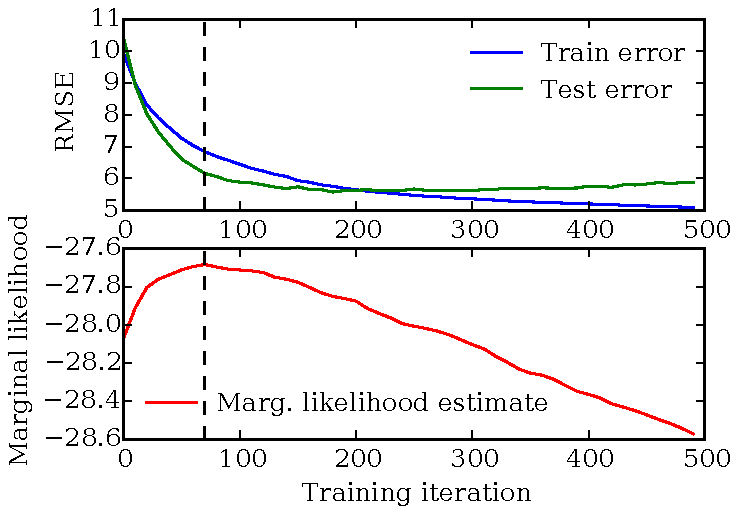
\includegraphics[width=1.15\columnwidth]{../experiments/2015_03_01_housing/2/marglik.pdf}
\end{column}
\end{columns}}


\frame[plain]{\frametitle{Experiments}
\begin{columns}
\hspace{-1cm}\begin{column}{6cm}
\begin{itemize} 
\item Choosing the number of hidden units
\item Top: Training and test-set likelihood as a function of the number of hidden units in the first layer of a neural network.
\item Bottom: Stochastic gradient descent marginal likelihood estimates.
\item Side result: Looks like inter-sample variance is low, surprisngly!
\end{itemize}
\end{column}
\begin{column}{5cm}
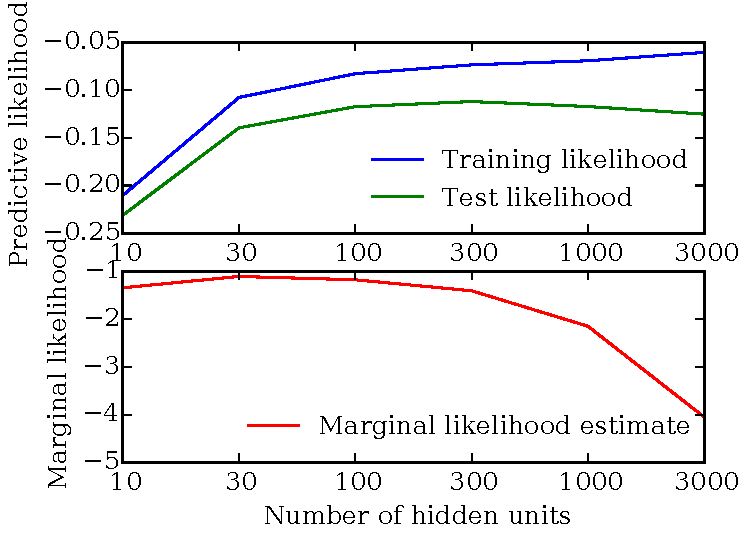
\includegraphics[width=1.15\columnwidth]{../experiments/2015_03_03_vary_width/7_hidden_units_higher_learnrate/vary_widths.pdf}
\end{column}
\end{columns}}



\frame[plain]{\frametitle{Experiments}
\begin{columns}
\hspace{-1cm}\begin{column}{6cm}
\begin{itemize} 
\item Choosing the number of hidden units
\item Top: Training and test-set likelihood as a function of the gradient threshold.
\item Marginal likelihood as a function of the gradient threshold.
A gradient threshold of zero corresponds to standard SGD.
\end{itemize}
\end{column}
\begin{column}{5cm}
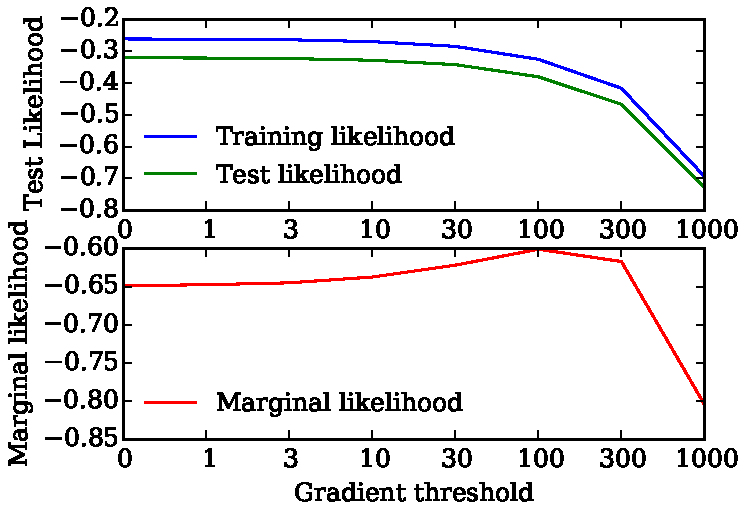
\includegraphics[width=1.15\columnwidth]{../experiments/2015_03_03_vary_width/5_grad_threshold/vary_widths.pdf}
\end{column}
\end{columns}}


\frame[plain]{\frametitle{Main Takeaways}
\begin{columns}
\hspace{-1cm}\begin{column}{6cm}
\begin{itemize} 
\item Optimization with random starts implies nonparametric intermediate distributions
\item Can estimate lower bound on model evidence during optimization using minibatches
\end{itemize}
\end{column}
\begin{column}{5cm}
\end{column}
\end{columns}}


\end{document}
